\documentclass[11pt,aspectratio=169]{beamer}
\usetheme{Madrid}

% ======================= PACKAGES =======================
\usepackage{graphicx}
\usepackage{booktabs}
\usepackage{adjustbox}
\usepackage{multicol}
\usepackage{amsmath}
\usepackage{amssymb}
\usepackage{tikz}
\usetikzlibrary{arrows,shapes,positioning,shadows,trees,calc,decorations.pathreplacing}
\usepackage{listings}
\usepackage{xcolor}

% ======================= COLOR DEFINITIONS =======================
% Primary color scheme: Blue/Teal for Digital Finance
\definecolor{dfblue}{RGB}{0,102,204}
\definecolor{dfteal}{RGB}{0,153,153}
\definecolor{dfcyan}{RGB}{51,187,204}
\definecolor{dflightblue}{RGB}{153,204,255}
\definecolor{dflightblue2}{RGB}{173,214,255}
\definecolor{dflightblue3}{RGB}{193,224,255}
\definecolor{dflightblue4}{RGB}{213,234,255}

% Accent colors for finance applications
\definecolor{dfgreen}{RGB}{44, 160, 44}
\definecolor{dfred}{RGB}{214, 39, 40}
\definecolor{dforange}{RGB}{255, 127, 14}
\definecolor{dfgray}{RGB}{127, 127, 127}

% Utility colors
\definecolor{lightgray}{RGB}{240, 240, 240}
\definecolor{midgray}{RGB}{180, 180, 180}
\definecolor{codebg}{RGB}{245, 245, 245}

% ======================= THEME CUSTOMIZATION =======================
\setbeamercolor{palette primary}{bg=dflightblue3,fg=dfblue}
\setbeamercolor{palette secondary}{bg=dflightblue2,fg=dfblue}
\setbeamercolor{palette tertiary}{bg=dfteal,fg=white}
\setbeamercolor{palette quaternary}{bg=dfblue,fg=white}

\setbeamercolor{structure}{fg=dfblue}
\setbeamercolor{section in toc}{fg=dfblue}
\setbeamercolor{subsection in toc}{fg=dfteal}
\setbeamercolor{title}{fg=dfblue}
\setbeamercolor{frametitle}{fg=dfblue,bg=dflightblue3}
\setbeamercolor{block title}{bg=dflightblue2,fg=dfblue}
\setbeamercolor{block body}{bg=dflightblue4,fg=black}

\setbeamertemplate{navigation symbols}{}
\setbeamertemplate{itemize items}[circle]
\setbeamertemplate{enumerate items}[default]
\setbeamersize{text margin left=8mm,text margin right=8mm}

% ======================= LISTINGS CONFIGURATION =======================
\lstdefinestyle{soliditystyle}{
    language=Java,
    basicstyle=\ttfamily\scriptsize,
    keywordstyle=\color{dfteal}\bfseries,
    stringstyle=\color{dforange},
    commentstyle=\color{dfgray}\itshape,
    numberstyle=\tiny\color{dfgray},
    numbers=left,
    numbersep=5pt,
    backgroundcolor=\color{codebg},
    showspaces=false,
    showstringspaces=false,
    showtabs=false,
    frame=single,
    rulecolor=\color{midgray},
    tabsize=2,
    captionpos=b,
    breaklines=true,
    breakatwhitespace=false,
    escapeinside={(*@}{@*)},
    xleftmargin=10pt,
    xrightmargin=10pt,
    morekeywords={pragma,solidity,contract,function,returns,public,private,view,pure,payable,address,uint256,mapping,event,modifier,require,emit,external,internal,msg,sender,value,memory,storage}
}

\lstdefinestyle{pythonstyle}{
    language=Python,
    basicstyle=\ttfamily\scriptsize,
    keywordstyle=\color{dfblue}\bfseries,
    stringstyle=\color{dforange},
    commentstyle=\color{dfgray}\itshape,
    numberstyle=\tiny\color{dfgray},
    numbers=left,
    numbersep=5pt,
    backgroundcolor=\color{codebg},
    showspaces=false,
    showstringspaces=false,
    showtabs=false,
    frame=single,
    rulecolor=\color{midgray},
    tabsize=4,
    captionpos=b,
    breaklines=true,
    breakatwhitespace=false,
    escapeinside={(*@}{@*)},
    xleftmargin=10pt,
    xrightmargin=10pt
}

\newcommand{\code}[1]{\texttt{\color{dfblue}#1}}

% ======================= CUSTOM COMMANDS =======================
\newcommand{\bottomnote}[1]{%
\vfill
\vspace{-2mm}
\textcolor{dflightblue2}{\rule{\textwidth}{0.4pt}}
\vspace{1mm}
\footnotesize
\textbf{#1}
}

\newcommand{\compactlist}{%
\setlength{\itemsep}{0pt}%
\setlength{\parskip}{0pt}%
\setlength{\parsep}{0pt}%
}

% ======================= FINANCE NOTATION MACROS =======================
\newcommand{\E}{\mathbb{E}}
\newcommand{\Var}{\mathrm{Var}}
\newcommand{\Cov}{\mathrm{Cov}}
\newcommand{\Prob}{\mathbb{P}}
\newcommand{\R}{\mathbb{R}}

% ======================= TIKZ STYLES =======================
\tikzstyle{process} = [rectangle, minimum width=3cm, minimum height=1cm, text centered, draw=dfblue, fill=dflightblue4, thick]
\tikzstyle{decision} = [diamond, minimum width=3cm, minimum height=1cm, text centered, draw=dfteal, fill=dflightblue4, thick]
\tikzstyle{arrow} = [thick,->,>=stealth,color=dfblue]
\tikzstyle{blockchain} = [rectangle, rounded corners, minimum width=2.5cm, minimum height=1cm, text centered, draw=dfteal, fill=dflightblue3, thick]
\tikzstyle{transaction} = [circle, minimum size=0.8cm, text centered, draw=dforange, fill=dflightblue4, thick]
\tikzstyle{smartcontract} = [rectangle, rounded corners, minimum width=2cm, minimum height=0.8cm, text centered, draw=dfblue, fill=dflightblue2, thick, font=\small]
\tikzstyle{pool} = [ellipse, minimum width=2.5cm, minimum height=1.5cm, text centered, draw=dfteal, fill=dflightblue3, thick]

% ======================= FOOTER TEMPLATE =======================
\setbeamertemplate{footline}{
    \hbox{\begin{beamercolorbox}[wd=\paperwidth,ht=2.5ex,dp=1ex,leftskip=.5em,rightskip=.5em]{author in head/foot}
    \tiny
    \textbf{Digital Finance} \hfill
    Joerg Osterrieder \hfill
    \insertdate \hfill
    Page \insertframenumber{} / \inserttotalframenumber
    \end{beamercolorbox}}
}

% ======================= SECTION DIVIDER TEMPLATE =======================
\AtBeginSection[]{
\begin{frame}[plain]
\vfill
\centering
\begin{beamercolorbox}[sep=12pt,center]{title}
\usebeamerfont{title}\LARGE\insertsection\par
\end{beamercolorbox}
\vfill
\end{frame}
}

% ======================= DOCUMENT INFO =======================
\title[Day 4: Programmable Finance]{Day 4: Programmable Finance}
\subtitle{Smart Contracts, DeFi, and Tokenization}
\author{Joerg Osterrieder}
\institute{Digital Finance Course}
\date{2025}

\begin{document}

% ======================= TITLE SLIDE =======================
\begin{frame}[plain]
\titlepage
\end{frame}

% ======================= TABLE OF CONTENTS =======================
\begin{frame}{Day 4 Overview}
\tableofcontents
\end{frame}

% ======================= DAY ARC SLIDE =======================
\begin{frame}{Day 4 Arc: From Mechanism to Systemic Impact}
\begin{center}
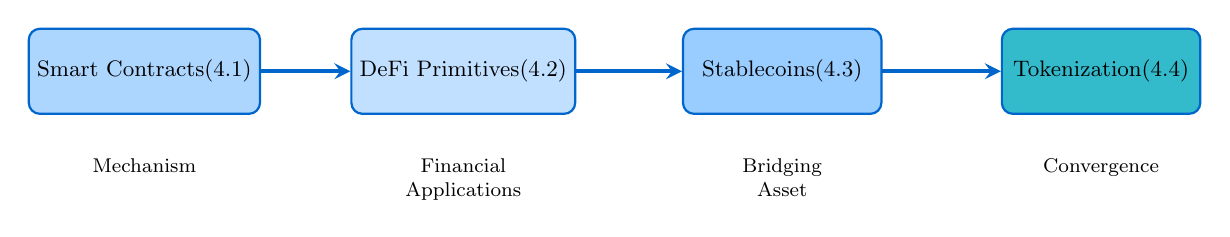
\begin{tikzpicture}[scale=0.9, transform shape]
    % Nodes
    \node[smartcontract, minimum width=2.8cm, minimum height=1.2cm] (sc) at (0,0) {Smart Contracts\\(4.1)};
    \node[smartcontract, minimum width=2.8cm, minimum height=1.2cm, fill=dflightblue3] (defi) at (4.5,0) {DeFi Primitives\\(4.2)};
    \node[smartcontract, minimum width=2.8cm, minimum height=1.2cm, fill=dflightblue] (stable) at (9,0) {Stablecoins\\(4.3)};
    \node[smartcontract, minimum width=2.8cm, minimum height=1.2cm, fill=dfcyan] (token) at (13.5,0) {Tokenization\\(4.4)};

    % Arrows
    \draw[arrow, line width=1.5pt] (sc) -- (defi);
    \draw[arrow, line width=1.5pt] (defi) -- (stable);
    \draw[arrow, line width=1.5pt] (stable) -- (token);

    % Labels below
    \node[below=0.5cm of sc, text width=2.5cm, align=center, font=\footnotesize] {Mechanism};
    \node[below=0.5cm of defi, text width=2.5cm, align=center, font=\footnotesize] {Financial\\Applications};
    \node[below=0.5cm of stable, text width=2.5cm, align=center, font=\footnotesize] {Bridging\\Asset};
    \node[below=0.5cm of token, text width=2.5cm, align=center, font=\footnotesize] {Convergence};
\end{tikzpicture}
\end{center}

\vspace{0.3cm}
\begin{block}{Day Purpose}
This is where crypto meets finance. Learn how smart contracts enable DeFi protocols that replicate (and sometimes improve upon) traditional financial services without intermediaries.
\end{block}
\end{frame}

% =====================================================================
% SECTION 4.1: SMART CONTRACTS
% =====================================================================
\section{4.1 Smart Contracts -- Code as Agreement}

\begin{frame}{What is a Smart Contract?}
\begin{columns}[T]
\begin{column}{0.55\textwidth}
\begin{block}{Definition}
A \textbf{smart contract} is a program stored on a blockchain that automatically executes when predetermined conditions are met.
\end{block}

\vspace{0.3cm}
\textbf{Key Properties:}
\begin{itemize}
    \item \textbf{Deterministic}: Same input always produces same output
    \item \textbf{Immutable}: Once deployed, code cannot be changed
    \item \textbf{Transparent}: Anyone can verify the code
    \item \textbf{Self-executing}: No intermediary needed
\end{itemize}
\end{column}

\begin{column}{0.42\textwidth}
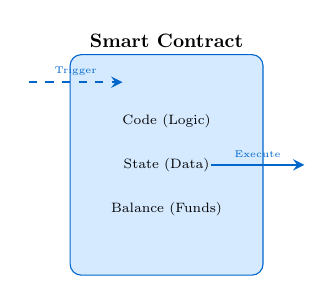
\begin{tikzpicture}[scale=0.7, transform shape]
    \node[rectangle, draw=dfblue, fill=dflightblue4, minimum width=3.5cm, minimum height=4cm, rounded corners] (contract) at (0,0) {};
    \node[above] at (contract.north) {\textbf{Smart Contract}};
    \node[align=center, font=\scriptsize] at (0,0.8) {Code (Logic)};
    \node[align=center, font=\scriptsize] at (0,0) {State (Data)};
    \node[align=center, font=\scriptsize] at (0,-0.8) {Balance (Funds)};

    \draw[arrow, dashed] (-2.5,1.5) -- (-0.8,1.5) node[midway, above, font=\tiny] {Trigger};
    \draw[arrow] (0.8,0) -- (2.5,0) node[midway, above, font=\tiny] {Execute};
\end{tikzpicture}
\end{column}
\end{columns}
\end{frame}

\begin{frame}{Traditional Contract vs. Smart Contract}
\begin{center}
\begin{tabular}{p{3.5cm}|p{4.5cm}|p{4.5cm}}
\toprule
\textbf{Aspect} & \textbf{Traditional Contract} & \textbf{Smart Contract} \\
\midrule
Enforcement & Courts, lawyers & Code execution \\
Trust & Counterparties, institutions & Cryptographic verification \\
Execution & Manual, subject to delay & Automatic, instant \\
Amendment & Negotiation, paperwork & Requires new deployment \\
Cost & High (intermediaries) & Low (gas fees only) \\
Transparency & Private documents & Public, auditable code \\
\bottomrule
\end{tabular}
\end{center}

\vspace{0.3cm}
\begin{alertblock}{Important Distinction}
``Trustless'' means you don't need to trust \textit{counterparties}---but you still need to trust the \textit{code}, the \textit{blockchain}, and the \textit{oracles}.
\end{alertblock}
\end{frame}

\begin{frame}{Smart Contract Execution Flow}
\begin{center}
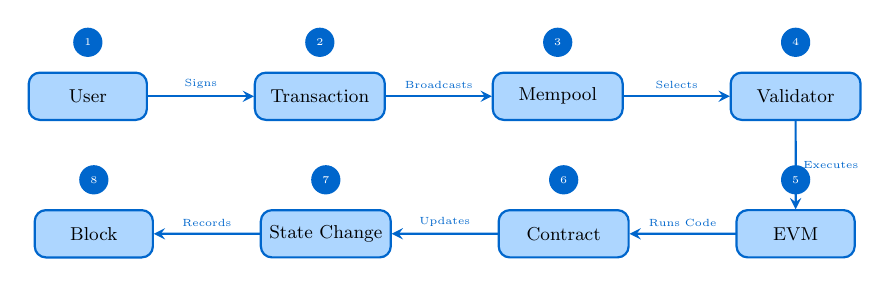
\begin{tikzpicture}[scale=0.75, transform shape, node distance=1.8cm]
    % Nodes
    \node[smartcontract, minimum width=2cm] (user) {User};
    \node[smartcontract, minimum width=2.2cm, right=of user] (tx) {Transaction};
    \node[smartcontract, minimum width=2.2cm, right=of tx] (mempool) {Mempool};
    \node[smartcontract, minimum width=2.2cm, right=of mempool] (validator) {Validator};
    \node[smartcontract, minimum width=2cm, below=1.5cm of validator] (evm) {EVM};
    \node[smartcontract, minimum width=2.2cm, left=of evm] (contract) {Contract};
    \node[smartcontract, minimum width=2.2cm, left=of contract] (state) {State Change};
    \node[smartcontract, minimum width=2cm, left=of state] (block) {Block};

    % Arrows
    \draw[arrow] (user) -- (tx) node[midway, above, font=\tiny] {Signs};
    \draw[arrow] (tx) -- (mempool) node[midway, above, font=\tiny] {Broadcasts};
    \draw[arrow] (mempool) -- (validator) node[midway, above, font=\tiny] {Selects};
    \draw[arrow] (validator) -- (evm) node[midway, right, font=\tiny] {Executes};
    \draw[arrow] (evm) -- (contract) node[midway, above, font=\tiny] {Runs Code};
    \draw[arrow] (contract) -- (state) node[midway, above, font=\tiny] {Updates};
    \draw[arrow] (state) -- (block) node[midway, above, font=\tiny] {Records};

    % Numbers
    \node[circle, fill=dfblue, text=white, font=\tiny] at ([yshift=0.5cm]user.north) {1};
    \node[circle, fill=dfblue, text=white, font=\tiny] at ([yshift=0.5cm]tx.north) {2};
    \node[circle, fill=dfblue, text=white, font=\tiny] at ([yshift=0.5cm]mempool.north) {3};
    \node[circle, fill=dfblue, text=white, font=\tiny] at ([yshift=0.5cm]validator.north) {4};
    \node[circle, fill=dfblue, text=white, font=\tiny] at ([yshift=0.5cm]evm.north) {5};
    \node[circle, fill=dfblue, text=white, font=\tiny] at ([yshift=0.5cm]contract.north) {6};
    \node[circle, fill=dfblue, text=white, font=\tiny] at ([yshift=0.5cm]state.north) {7};
    \node[circle, fill=dfblue, text=white, font=\tiny] at ([yshift=0.5cm]block.north) {8};
\end{tikzpicture}
\end{center}

\vspace{0.2cm}
\begin{enumerate}
\footnotesize
    \item User creates and signs transaction calling contract function
    \item Transaction broadcast to network
    \item Transaction waits in mempool
    \item Validator selects transaction for block
    \item Ethereum Virtual Machine (EVM) executes bytecode
    \item Contract logic runs with provided inputs
    \item State changes recorded (balances, storage)
    \item Changes finalized in blockchain block
\end{enumerate}
\end{frame}

\begin{frame}[fragile]{Anatomy of a Smart Contract (Solidity)}
\begin{lstlisting}[style=soliditystyle]
// SPDX-License-Identifier: MIT
pragma solidity ^0.8.0;

contract SimpleEscrow {
    address public buyer;
    address public seller;
    uint256 public amount;
    bool public released;

    constructor(address _seller) payable {
        buyer = msg.sender;
        seller = _seller;
        amount = msg.value;
    }

    function release() external {
        require(msg.sender == buyer, "Only buyer can release");
        require(!released, "Already released");
        released = true;
        payable(seller).transfer(amount);
    }
}
\end{lstlisting}

\bottomnote{Hands-on: NB08 -- Interact with smart contracts on testnet}
\end{frame}

\begin{frame}{The Oracle Problem}
\begin{columns}[T]
\begin{column}{0.48\textwidth}
\begin{block}{The Challenge}
Smart contracts cannot access external data---they only know what's on the blockchain.
\end{block}

\vspace{0.3cm}
\textbf{Examples requiring oracles:}
\begin{itemize}
    \item Price feeds (ETH/USD)
    \item Weather data for insurance
    \item Sports scores for betting
    \item Real-world asset values
\end{itemize}
\end{column}

\begin{column}{0.48\textwidth}
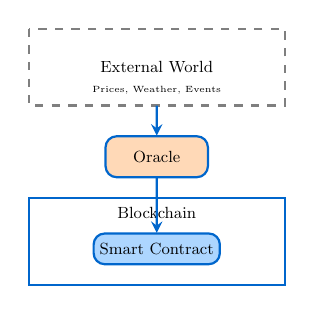
\begin{tikzpicture}[scale=0.65, transform shape]
    % External world
    \draw[dashed, thick, dfgray] (-2.5, 2.5) rectangle (2.5, 1);
    \node[font=\small] at (0, 1.75) {External World};
    \node[font=\tiny] at (0, 1.3) {Prices, Weather, Events};

    % Oracle
    \node[smartcontract, fill=dforange!30, minimum width=2cm] (oracle) at (0, 0) {Oracle};

    % Blockchain
    \draw[thick, dfblue] (-2.5, -0.8) rectangle (2.5, -2.5);
    \node[font=\small] at (0, -1.1) {Blockchain};
    \node[smartcontract, minimum width=1.8cm, minimum height=0.6cm] (sc) at (0, -1.8) {Smart Contract};

    % Arrows
    \draw[arrow] (0, 1) -- (oracle);
    \draw[arrow] (oracle) -- (sc);
\end{tikzpicture}

\vspace{0.2cm}
\textbf{Solutions:}
\begin{itemize}
    \item Chainlink (decentralized)
    \item API3, Band Protocol
    \item Optimistic oracles (UMA)
\end{itemize}
\end{column}
\end{columns}
\end{frame}

\begin{frame}{Smart Contract Risks and Limitations}
\begin{columns}[T]
\begin{column}{0.48\textwidth}
\textbf{Technical Risks:}
\begin{itemize}
    \item \textbf{Bugs}: Code is immutable---bugs are forever
    \item \textbf{Reentrancy}: The DAO hack (\$60M, 2016)
    \item \textbf{Integer overflow}: Pre-0.8 Solidity
    \item \textbf{Oracle manipulation}: Flash loan attacks
    \item \textbf{Front-running}: MEV extraction
\end{itemize}

\vspace{0.3cm}
\textbf{Gas Considerations:}
\begin{itemize}
    \item Every operation costs gas
    \item Complex logic = expensive
    \item Storage is most expensive
    \item Out-of-gas reverts transaction
\end{itemize}
\end{column}

\begin{column}{0.48\textwidth}
\textbf{Design Limitations:}
\begin{itemize}
    \item Cannot handle ambiguity
    \item No subjective judgments
    \item Cannot initiate actions
    \item Limited to on-chain data
\end{itemize}

\vspace{0.3cm}
\begin{alertblock}{The Immutability Paradox}
Immutability provides security guarantees but makes bug fixes impossible. Solutions: proxy patterns, upgradeable contracts---but these reintroduce trust assumptions.
\end{alertblock}
\end{column}
\end{columns}
\end{frame}

\begin{frame}{What ``Trustless'' Really Means}
\begin{center}
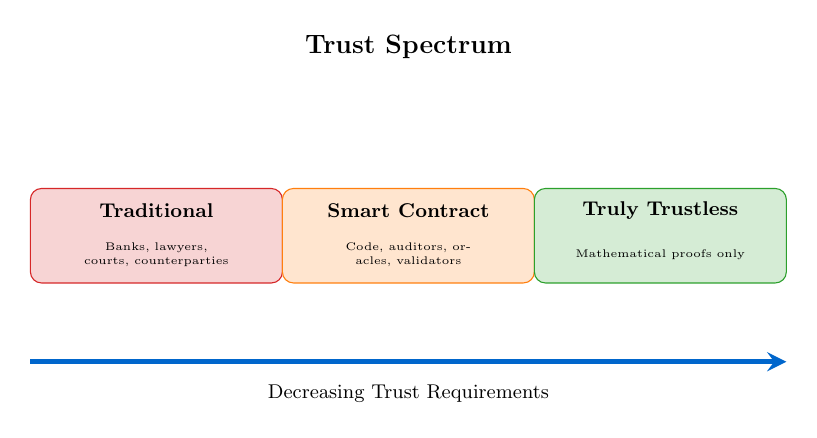
\begin{tikzpicture}[scale=0.8, transform shape]
    % Title
    \node[font=\large\bfseries] at (0, 3) {Trust Spectrum};

    % Traditional
    \node[rectangle, draw=dfred, fill=dfred!20, minimum width=4cm, minimum height=1.5cm, rounded corners] (trad) at (-4, 0) {};
    \node[font=\small\bfseries] at (-4, 0.4) {Traditional};
    \node[font=\tiny, text width=3.5cm, align=center] at (-4, -0.3) {Banks, lawyers, courts, counterparties};

    % Smart Contract
    \node[rectangle, draw=dforange, fill=dforange!20, minimum width=4cm, minimum height=1.5cm, rounded corners] (smart) at (0, 0) {};
    \node[font=\small\bfseries] at (0, 0.4) {Smart Contract};
    \node[font=\tiny, text width=3.5cm, align=center] at (0, -0.3) {Code, auditors, oracles, validators};

    % Theoretical
    \node[rectangle, draw=dfgreen, fill=dfgreen!20, minimum width=4cm, minimum height=1.5cm, rounded corners] (theory) at (4, 0) {};
    \node[font=\small\bfseries] at (4, 0.4) {Truly Trustless};
    \node[font=\tiny, text width=3.5cm, align=center] at (4, -0.3) {Mathematical proofs only};

    % Arrow
    \draw[arrow, line width=2pt] (-6, -2) -- (6, -2);
    \node[font=\small] at (0, -2.5) {Decreasing Trust Requirements};
\end{tikzpicture}
\end{center}

\vspace{0.3cm}
\begin{block}{Key Insight}
Smart contracts shift trust from \textit{institutions} to \textit{code and cryptography}. This is valuable---but it's a different kind of trust, not the absence of trust.
\end{block}
\end{frame}

\begin{frame}{Key Competency Check: Smart Contracts}
\begin{block}{You should be able to:}
\begin{enumerate}
    \item Explain how a smart contract executes on a blockchain
    \item Define what ``trustless'' means (and doesn't mean)
    \item Identify key limitations: oracle problem, immutability risks
    \item Read and understand the logic of a simple contract
\end{enumerate}
\end{block}

\vspace{0.5cm}
\begin{center}
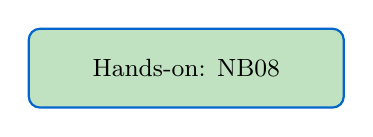
\begin{tikzpicture}
    \node[smartcontract, minimum width=4cm, minimum height=1cm, fill=dfgreen!30] {Hands-on: NB08};
\end{tikzpicture}
\end{center}

\textbf{NB08}: Interact with a simple smart contract (token or escrow) on testnet---call functions and observe state changes.
\end{frame}

% =====================================================================
% SECTION 4.2: DEFI PRIMITIVES
% =====================================================================
\section{4.2 DeFi Primitives -- Lending, Trading, and Yield}

\begin{frame}{What is DeFi?}
\begin{columns}[T]
\begin{column}{0.55\textwidth}
\begin{block}{Definition}
\textbf{Decentralized Finance (DeFi)} refers to financial services built on public blockchains that operate without traditional intermediaries.
\end{block}

\vspace{0.3cm}
\textbf{Core Principles:}
\begin{itemize}
    \item \textbf{Permissionless}: Anyone can participate
    \item \textbf{Non-custodial}: Users control their assets
    \item \textbf{Transparent}: All code and transactions public
    \item \textbf{Composable}: Protocols can be combined
\end{itemize}
\end{column}

\begin{column}{0.42\textwidth}
\textbf{DeFi Ecosystem (2024):}
\begin{itemize}
    \item Total Value Locked: \$50B+
    \item Daily trading volume: \$2B+
    \item Active protocols: 500+
    \item Supported chains: 50+
\end{itemize}

\vspace{0.3cm}
\textbf{Major Categories:}
\begin{itemize}
    \item Decentralized Exchanges
    \item Lending Protocols
    \item Derivatives
    \item Yield Aggregators
\end{itemize}
\end{column}
\end{columns}
\end{frame}

\begin{frame}{DeFi vs. Traditional Finance}
\begin{center}
\begin{tabular}{p{3cm}|p{5cm}|p{5cm}}
\toprule
\textbf{Feature} & \textbf{Traditional Finance} & \textbf{DeFi} \\
\midrule
Access & KYC, credit checks & Wallet address only \\
Hours & Business hours, T+2 settlement & 24/7/365, instant \\
Custody & Institutions hold assets & User self-custody \\
Transparency & Private ledgers & Public blockchain \\
Innovation & Regulatory approval needed & Permissionless deployment \\
Risk & Counterparty, institution & Smart contract, oracle \\
\bottomrule
\end{tabular}
\end{center}

\vspace{0.3cm}
\begin{alertblock}{The Composability Advantage}
DeFi protocols are like ``money legos''---they can be combined in ways their creators never anticipated. A flash loan can be used in an arbitrage that spans 5 different protocols in a single transaction.
\end{alertblock}
\end{frame}

\begin{frame}{Automated Market Makers (AMMs)}
\begin{columns}[T]
\begin{column}{0.48\textwidth}
\textbf{Traditional Exchange:}
\begin{itemize}
    \item Order book with bids/asks
    \item Market makers provide liquidity
    \item Requires active management
    \item Centralized matching engine
\end{itemize}

\vspace{0.3cm}
\textbf{AMM Innovation:}
\begin{itemize}
    \item No order book needed
    \item Liquidity pools replace market makers
    \item Algorithmic pricing
    \item Anyone can provide liquidity
\end{itemize}
\end{column}

\begin{column}{0.48\textwidth}
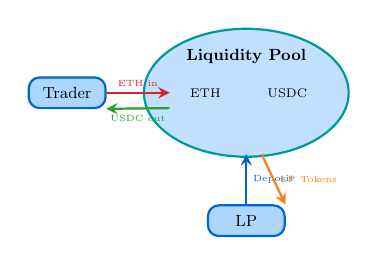
\begin{tikzpicture}[scale=0.65, transform shape]
    % Pool
    \node[pool, minimum width=4cm, minimum height=2.5cm] (pool) at (0,0) {};
    \node[font=\small\bfseries] at (0, 0.7) {Liquidity Pool};
    \node[font=\scriptsize] at (-0.8, 0) {ETH};
    \node[font=\scriptsize] at (0.8, 0) {USDC};

    % Trader
    \node[smartcontract, minimum width=1.5cm, minimum height=0.6cm] (trader) at (-3.5, 0) {Trader};

    % LP
    \node[smartcontract, minimum width=1.5cm, minimum height=0.6cm] (lp) at (0, -2.5) {LP};

    % Arrows
    \draw[arrow, dfred] (trader) -- (-1.5, 0) node[midway, above, font=\tiny] {ETH in};
    \draw[arrow, dfgreen] (-1.5, -0.3) -- (trader.south east) node[midway, below, font=\tiny] {USDC out};

    \draw[arrow, dfblue] (lp) -- (0, -1.2) node[midway, right, font=\tiny] {Deposit};
    \draw[arrow, dforange] (0.3, -1.2) -- (lp.north east) node[midway, right, font=\tiny] {LP Tokens};
\end{tikzpicture}
\end{column}
\end{columns}

\vspace{0.2cm}
\textbf{Key Protocols:} Uniswap, SushiSwap, Curve, Balancer
\end{frame}

\begin{frame}{Constant Product Formula: $x \cdot y = k$}
\begin{columns}[T]
\begin{column}{0.45\textwidth}
\begin{block}{The Core Equation}
\[
x \cdot y = k
\]
\begin{itemize}
    \item $x$ = Token A reserves
    \item $y$ = Token B reserves
    \item $k$ = Constant (invariant)
\end{itemize}
\end{block}

\vspace{0.2cm}
\textbf{Price Determination:}
\[
\text{Price of A in B} = \frac{y}{x}
\]

\textbf{After swap of $\Delta x$:}
\[
\Delta y = y - \frac{k}{x + \Delta x}
\]
\end{column}

\begin{column}{0.52\textwidth}
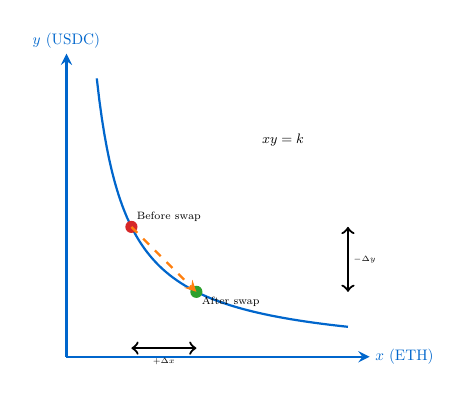
\begin{tikzpicture}[scale=0.55, transform shape]
    % Axes
    \draw[arrow] (0,0) -- (7,0) node[right] {$x$ (ETH)};
    \draw[arrow] (0,0) -- (0,7) node[above] {$y$ (USDC)};

    % Curve xy = k
    \draw[thick, dfblue, domain=0.7:6.5, samples=100] plot (\x, {4.5/\x});

    % Points
    \fill[dfred] (1.5, 3) circle (4pt);
    \node[above right, font=\scriptsize] at (1.5, 3) {Before swap};

    \fill[dfgreen] (3, 1.5) circle (4pt);
    \node[below right, font=\scriptsize] at (3, 1.5) {After swap};

    % Trade arrow
    \draw[arrow, dforange, thick, dashed] (1.5, 3) -- (3, 1.5);

    % Annotations
    \draw[<->, thick] (1.5, 0.2) -- (3, 0.2);
    \node[below, font=\tiny] at (2.25, 0.1) {$+\Delta x$};

    \draw[<->, thick] (6.5, 1.5) -- (6.5, 3);
    \node[right, font=\tiny] at (6.5, 2.25) {$-\Delta y$};

    % Label
    \node[font=\small] at (5, 5) {$xy = k$};
\end{tikzpicture}
\end{column}
\end{columns}

\vspace{0.2cm}
\begin{alertblock}{Price Impact}
Larger trades move further along the curve, resulting in worse prices. This is called \textbf{slippage} or \textbf{price impact}.
\end{alertblock}
\end{frame}

\begin{frame}{AMM Numerical Example}
\begin{block}{Initial Pool State}
\begin{itemize}
    \item 100 ETH + 300,000 USDC
    \item $k = 100 \times 300,000 = 30,000,000$
    \item Price: 1 ETH = 3,000 USDC
\end{itemize}
\end{block}

\textbf{Trader swaps 10 ETH for USDC:}
\begin{align*}
\text{New ETH reserves:} \quad x' &= 100 + 10 = 110 \\
\text{New USDC reserves:} \quad y' &= \frac{30,000,000}{110} = 272,727.27 \\
\text{USDC received:} \quad \Delta y &= 300,000 - 272,727.27 = 27,272.73
\end{align*}

\begin{alertblock}{Price Impact Analysis}
\begin{itemize}
    \item Expected (no impact): $10 \times 3,000 = 30,000$ USDC
    \item Actual received: 27,272.73 USDC
    \item Slippage: $\frac{30,000 - 27,272.73}{30,000} = 9.09\%$
    \item New price: $\frac{272,727.27}{110} = 2,479.34$ USDC/ETH
\end{itemize}
\end{alertblock}
\end{frame}

\begin{frame}{Liquidity Pool Mechanics}
\begin{center}
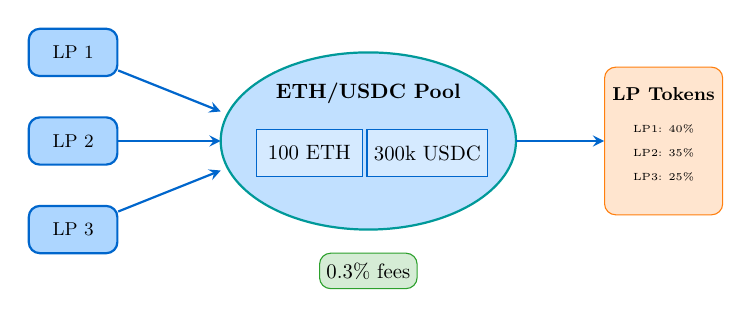
\begin{tikzpicture}[scale=0.75, transform shape]
    % Pool
    \node[pool, minimum width=5cm, minimum height=3cm, fill=dflightblue3] (pool) at (0,0) {};
    \node[font=\bfseries] at (0, 0.8) {ETH/USDC Pool};

    % Reserves
    \node[rectangle, draw=dfblue, fill=dflightblue4, minimum width=1.8cm, minimum height=0.8cm] at (-1, -0.2) {100 ETH};
    \node[rectangle, draw=dfblue, fill=dflightblue4, minimum width=1.8cm, minimum height=0.8cm] at (1, -0.2) {300k USDC};

    % LPs
    \node[smartcontract, minimum width=1.5cm] (lp1) at (-5, 1.5) {LP 1};
    \node[smartcontract, minimum width=1.5cm] (lp2) at (-5, 0) {LP 2};
    \node[smartcontract, minimum width=1.5cm] (lp3) at (-5, -1.5) {LP 3};

    % LP tokens
    \node[rectangle, draw=dforange, fill=dforange!20, minimum width=2cm, minimum height=2.5cm, rounded corners] (lptokens) at (5, 0) {};
    \node[font=\small\bfseries] at (5, 0.8) {LP Tokens};
    \node[font=\tiny] at (5, 0.2) {LP1: 40\%};
    \node[font=\tiny] at (5, -0.2) {LP2: 35\%};
    \node[font=\tiny] at (5, -0.6) {LP3: 25\%};

    % Arrows
    \draw[arrow] (lp1) -- (-2.5, 0.5);
    \draw[arrow] (lp2) -- (-2.5, 0);
    \draw[arrow] (lp3) -- (-2.5, -0.5);

    \draw[arrow] (2.5, 0) -- (lptokens);

    % Fees
    \node[rectangle, draw=dfgreen, fill=dfgreen!20, minimum width=1.5cm, minimum height=0.6cm, rounded corners] at (0, -2.2) {0.3\% fees};
\end{tikzpicture}
\end{center}

\textbf{LP Token Mechanics:}
\begin{itemize}
    \item LP tokens represent proportional claim on pool reserves
    \item Fees accumulate in pool, increasing LP token value
    \item Withdrawal returns proportional share of \textit{current} reserves
\end{itemize}
\end{frame}

\begin{frame}{Impermanent Loss Explained}
\begin{block}{Definition}
\textbf{Impermanent Loss (IL)} is the difference between holding assets in a liquidity pool vs. simply holding them in your wallet.
\end{block}

\textbf{Why it happens:}
\begin{enumerate}
    \item You deposit equal value: 1 ETH (\$3,000) + 3,000 USDC
    \item ETH price doubles to \$6,000
    \item Arbitrageurs rebalance the pool
    \item Your LP position: 0.707 ETH + 4,243 USDC = \$8,485
    \item If you had just held: 1 ETH + 3,000 USDC = \$9,000
    \item \textbf{Impermanent Loss: \$515 (5.72\%)}
\end{enumerate}

\vspace{0.2cm}
\begin{alertblock}{Key Insight}
Loss is ``impermanent'' because if prices return to original levels, the loss disappears. It becomes \textit{permanent} when you withdraw at different prices.
\end{alertblock}
\end{frame}

\begin{frame}{Impermanent Loss Formula and Visualization}
\begin{columns}[T]
\begin{column}{0.45\textwidth}
\textbf{IL Formula:}
\[
IL = \frac{2\sqrt{r}}{1+r} - 1
\]
where $r = \frac{P_1}{P_0}$ (price ratio)

\vspace{0.3cm}
\begin{tabular}{cc}
\toprule
\textbf{Price Change} & \textbf{IL} \\
\midrule
1.25x (25\% up) & 0.6\% \\
1.50x (50\% up) & 2.0\% \\
2x (100\% up) & 5.7\% \\
3x (200\% up) & 13.4\% \\
4x (300\% up) & 20.0\% \\
5x (400\% up) & 25.5\% \\
\bottomrule
\end{tabular}
\end{column}

\begin{column}{0.52\textwidth}
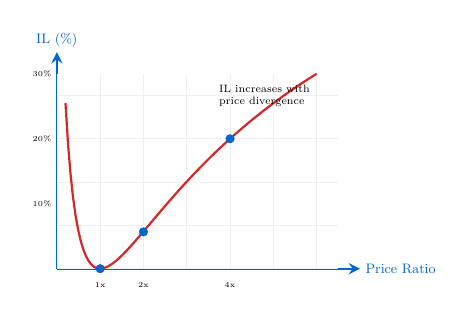
\begin{tikzpicture}[scale=0.55, transform shape]
    % Axes
    \draw[arrow] (0,0) -- (7,0) node[right, font=\small] {Price Ratio};
    \draw[arrow] (0,0) -- (0,5) node[above, font=\small] {IL (\%)};

    % Grid
    \draw[very thin, lightgray] (0,0) grid (6.5,4.5);

    % IL curve
    \draw[thick, dfred, domain=0.2:6, samples=100] plot (\x, {(1 - 2*sqrt(\x)/(1+\x))*15});

    % Points
    \fill[dfblue] (1, 0) circle (3pt);
    \node[below, font=\tiny] at (1, -0.2) {1x};

    \fill[dfblue] (2, 0.85) circle (3pt);
    \node[below, font=\tiny] at (2, -0.2) {2x};

    \fill[dfblue] (4, 3) circle (3pt);
    \node[below, font=\tiny] at (4, -0.2) {4x};

    % Y-axis labels
    \node[left, font=\tiny] at (0, 1.5) {10\%};
    \node[left, font=\tiny] at (0, 3) {20\%};
    \node[left, font=\tiny] at (0, 4.5) {30\%};

    % Annotation
    \node[font=\scriptsize, text width=2.5cm] at (5, 4) {IL increases with price divergence};
\end{tikzpicture}
\end{column}
\end{columns}

\vspace{0.2cm}
\textbf{Mitigating IL:}
\begin{itemize}
    \item Provide liquidity to correlated pairs (stablecoin-stablecoin)
    \item Choose pools with high trading volume (fees offset IL)
    \item Use concentrated liquidity (Uniswap V3)
\end{itemize}
\end{frame}

\begin{frame}{DeFi Lending: How It Works}
\begin{center}
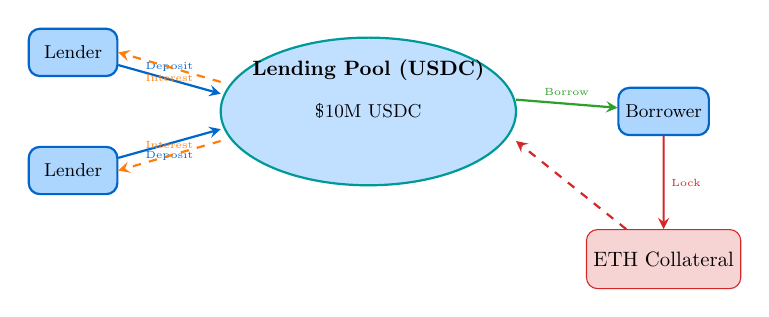
\begin{tikzpicture}[scale=0.75, transform shape]
    % Lending Pool
    \node[pool, minimum width=5cm, minimum height=2.5cm] (pool) at (0,0) {};
    \node[font=\bfseries] at (0, 0.7) {Lending Pool (USDC)};
    \node[font=\small] at (0, 0) {\$10M USDC};

    % Lenders
    \node[smartcontract, minimum width=1.5cm] (lend1) at (-5, 1) {Lender};
    \node[smartcontract, minimum width=1.5cm] (lend2) at (-5, -1) {Lender};

    % Borrowers
    \node[smartcontract, minimum width=1.5cm] (borrow) at (5, 0) {Borrower};

    % Collateral box
    \node[rectangle, draw=dfred, fill=dfred!20, minimum width=2cm, minimum height=1cm, rounded corners] (collat) at (5, -2.5) {ETH Collateral};

    % Arrows
    \draw[arrow, dfblue] (lend1) -- (-2.5, 0.3) node[midway, above, font=\tiny] {Deposit};
    \draw[arrow, dfblue] (lend2) -- (-2.5, -0.3) node[midway, below, font=\tiny] {Deposit};

    \draw[arrow, dfgreen] (2.5, 0.2) -- (borrow) node[midway, above, font=\tiny] {Borrow};
    \draw[arrow, dfred] (borrow) -- (collat) node[midway, right, font=\tiny] {Lock};
    \draw[arrow, dfred, dashed] (collat) -- (2.5, -0.5);

    % Interest arrows
    \draw[arrow, dforange, dashed] (-2.5, 0.5) -- (lend1.east) node[midway, below, font=\tiny] {Interest};
    \draw[arrow, dforange, dashed] (-2.5, -0.5) -- (lend2.east) node[midway, above, font=\tiny] {Interest};
\end{tikzpicture}
\end{center}

\textbf{Key Mechanics:}
\begin{itemize}
    \item \textbf{Over-collateralization}: Borrow \$1,000 requires \$1,500+ collateral
    \item \textbf{Algorithmic rates}: Interest adjusts with utilization
    \item \textbf{Liquidation}: If collateral falls below threshold, anyone can liquidate
\end{itemize}
\end{frame}

\begin{frame}{Algorithmic Interest Rates}
\begin{columns}[T]
\begin{column}{0.45\textwidth}
\textbf{Utilization Rate:}
\[
U = \frac{\text{Borrowed}}{\text{Supplied}}
\]

\textbf{Borrow Rate (kinked model):}
\[
R_{\text{borrow}} =
\begin{cases}
R_0 + U \cdot R_{\text{slope1}} & U < U_{\text{optimal}} \\
R_0 + U_{\text{opt}} \cdot R_1 + \\
\quad (U - U_{\text{opt}}) \cdot R_2 & U \geq U_{\text{optimal}}
\end{cases}
\]

\textbf{Supply Rate:}
\[
R_{\text{supply}} = R_{\text{borrow}} \times U \times (1 - \text{fee})
\]
\end{column}

\begin{column}{0.52\textwidth}
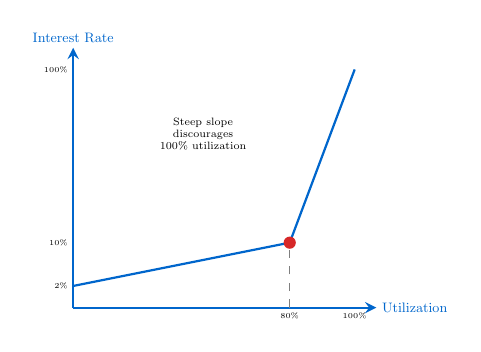
\begin{tikzpicture}[scale=0.55, transform shape]
    % Axes
    \draw[arrow] (0,0) -- (7,0) node[right, font=\small] {Utilization};
    \draw[arrow] (0,0) -- (0,6) node[above, font=\small] {Interest Rate};

    % Kinked curve
    \draw[thick, dfblue] (0, 0.5) -- (5, 1.5);
    \draw[thick, dfblue] (5, 1.5) -- (6.5, 5.5);

    % Optimal point
    \draw[dashed, dfgray] (5, 0) -- (5, 1.5);
    \fill[dfred] (5, 1.5) circle (4pt);

    % Labels
    \node[below, font=\tiny] at (5, 0) {80\%};
    \node[below, font=\tiny] at (6.5, 0) {100\%};
    \node[left, font=\tiny] at (0, 0.5) {2\%};
    \node[left, font=\tiny] at (0, 1.5) {10\%};
    \node[left, font=\tiny] at (0, 5.5) {100\%};

    % Annotation
    \node[font=\scriptsize, text width=2cm, align=center] at (3, 4) {Steep slope\\discourages\\100\% utilization};
\end{tikzpicture}
\end{column}
\end{columns}

\vspace{0.2cm}
\textbf{Key Protocols:} Aave, Compound, MakerDAO

\bottomnote{Hands-on: NB09 -- Simulate AMM and observe impermanent loss}
\end{frame}

\begin{frame}{Flash Loans: Innovation or Attack Vector?}
\begin{block}{Definition}
A \textbf{flash loan} is an uncollateralized loan that must be borrowed and repaid within a single transaction.
\end{block}

\begin{center}
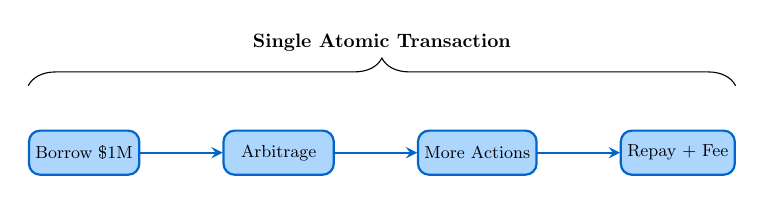
\begin{tikzpicture}[scale=0.7, transform shape, node distance=1.5cm]
    \node[smartcontract] (borrow) {Borrow \$1M};
    \node[smartcontract, right=of borrow] (use1) {Arbitrage};
    \node[smartcontract, right=of use1] (use2) {More Actions};
    \node[smartcontract, right=of use2] (repay) {Repay + Fee};

    \draw[arrow] (borrow) -- (use1);
    \draw[arrow] (use1) -- (use2);
    \draw[arrow] (use2) -- (repay);

    % Single transaction bracket
    \draw[decorate, decoration={brace, amplitude=10pt}]
        ([yshift=0.8cm]borrow.north west) -- ([yshift=0.8cm]repay.north east)
        node[midway, above=0.5cm] {\textbf{Single Atomic Transaction}};
\end{tikzpicture}
\end{center}

\textbf{Legitimate Uses:} Arbitrage, collateral swaps, self-liquidation

\textbf{Attack Uses:} Oracle manipulation, governance attacks, protocol exploits

\begin{alertblock}{The Double-Edged Sword}
Flash loans democratize access to capital but have enabled over \$500M in DeFi exploits.
\end{alertblock}
\end{frame}

\begin{frame}{Key Competency Check: DeFi Primitives}
\begin{block}{You should be able to:}
\begin{enumerate}
    \item Explain how an AMM prices assets using $x \cdot y = k$
    \item Calculate price impact/slippage for a given trade
    \item Understand how DeFi lending determines interest rates algorithmically
    \item Calculate impermanent loss for price changes
\end{enumerate}
\end{block}

\vspace{0.5cm}
\begin{center}
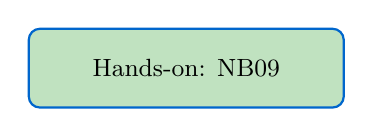
\begin{tikzpicture}
    \node[smartcontract, minimum width=4cm, minimum height=1cm, fill=dfgreen!30] {Hands-on: NB09};
\end{tikzpicture}
\end{center}

\textbf{NB09}: Simulate a constant-product AMM---provide liquidity, execute swaps, observe price impact and impermanent loss.
\end{frame}

% =====================================================================
% SECTION 4.3: STABLECOINS
% =====================================================================
\section{4.3 Stablecoins -- The Bridge Between Two Worlds}

\begin{frame}{Why Stablecoins Matter}
\begin{columns}[T]
\begin{column}{0.55\textwidth}
\begin{block}{Definition}
\textbf{Stablecoins} are cryptocurrencies designed to maintain a stable value relative to a reference asset (typically USD).
\end{block}

\vspace{0.3cm}
\textbf{The Problem They Solve:}
\begin{itemize}
    \item Crypto volatility makes it unsuitable for payments
    \item Traditional banking hours and fees
    \item Need for on-chain ``cash'' in DeFi
    \item Cross-border payment friction
\end{itemize}
\end{column}

\begin{column}{0.42\textwidth}
\textbf{Market Size (2024):}
\begin{itemize}
    \item Total supply: \$170B+
    \item Daily volume: \$50B+
    \item Surpasses Visa in some metrics
\end{itemize}

\vspace{0.3cm}
\textbf{Use Cases:}
\begin{itemize}
    \item Trading pairs on exchanges
    \item DeFi collateral and lending
    \item Remittances
    \item Savings in dollarized economies
\end{itemize}
\end{column}
\end{columns}
\end{frame}

\begin{frame}{Stablecoin Design Taxonomy}
\begin{center}
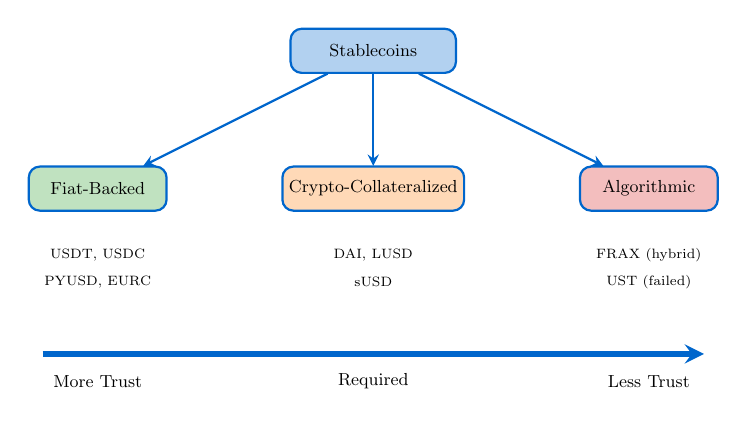
\begin{tikzpicture}[scale=0.7, transform shape]
    % Root
    \node[smartcontract, minimum width=3cm, fill=dfblue!30] (root) at (0, 3) {Stablecoins};

    % Three types
    \node[smartcontract, minimum width=2.5cm, fill=dfgreen!30] (fiat) at (-5, 0.5) {Fiat-Backed};
    \node[smartcontract, minimum width=2.5cm, fill=dforange!30] (crypto) at (0, 0.5) {Crypto-Collateralized};
    \node[smartcontract, minimum width=2.5cm, fill=dfred!30] (algo) at (5, 0.5) {Algorithmic};

    % Examples
    \node[font=\scriptsize] at (-5, -0.7) {USDT, USDC};
    \node[font=\scriptsize] at (-5, -1.2) {PYUSD, EURC};

    \node[font=\scriptsize] at (0, -0.7) {DAI, LUSD};
    \node[font=\scriptsize] at (0, -1.2) {sUSD};

    \node[font=\scriptsize] at (5, -0.7) {FRAX (hybrid)};
    \node[font=\scriptsize] at (5, -1.2) {\sout{UST} (failed)};

    % Arrows
    \draw[arrow] (root) -- (fiat);
    \draw[arrow] (root) -- (crypto);
    \draw[arrow] (root) -- (algo);

    % Trust spectrum
    \draw[arrow, line width=2pt] (-6, -2.5) -- (6, -2.5);
    \node[font=\small] at (-5, -3) {More Trust};
    \node[font=\small] at (5, -3) {Less Trust};
    \node[font=\small] at (0, -3) {Required};
\end{tikzpicture}
\end{center}
\end{frame}

\begin{frame}{Fiat-Backed Stablecoins}
\begin{columns}[T]
\begin{column}{0.48\textwidth}
\textbf{How It Works:}
\begin{enumerate}
    \item User sends \$1 to issuer
    \item Issuer holds \$1 in reserves
    \item Issuer mints 1 stablecoin
    \item User can redeem anytime
\end{enumerate}

\vspace{0.3cm}
\textbf{Examples:}
\begin{itemize}
    \item \textbf{USDT} (Tether): \$110B, largest
    \item \textbf{USDC} (Circle): \$35B, regulated
    \item \textbf{PYUSD} (PayPal): Newest entrant
\end{itemize}
\end{column}

\begin{column}{0.48\textwidth}
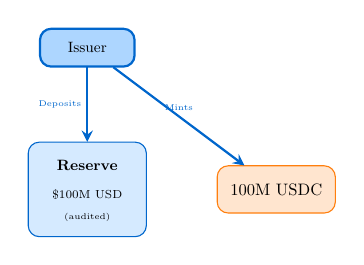
\begin{tikzpicture}[scale=0.6, transform shape]
    % Bank
    \node[rectangle, draw=dfblue, fill=dflightblue4, minimum width=2.5cm, minimum height=2cm, rounded corners] (bank) at (0, 0) {};
    \node[font=\small\bfseries] at (0, 0.5) {Reserve};
    \node[font=\scriptsize] at (0, -0.1) {\$100M USD};
    \node[font=\tiny] at (0, -0.6) {(audited)};

    % Issuer
    \node[smartcontract, minimum width=2cm] (issuer) at (0, 3) {Issuer};

    % Supply
    \node[rectangle, draw=dforange, fill=dforange!20, minimum width=2.5cm, minimum height=1cm, rounded corners] (supply) at (4, 0) {100M USDC};

    % Arrows
    \draw[arrow] (issuer) -- (bank) node[midway, left, font=\tiny] {Deposits};
    \draw[arrow] (issuer) -- (supply) node[midway, above, font=\tiny] {Mints};
\end{tikzpicture}

\vspace{0.3cm}
\textbf{Risks:}
\begin{itemize}
    \item Centralized---can freeze funds
    \item Reserve quality concerns
    \item Regulatory uncertainty
    \item Banking system dependence
\end{itemize}
\end{column}
\end{columns}
\end{frame}

\begin{frame}{Crypto-Collateralized Stablecoins}
\begin{columns}[T]
\begin{column}{0.48\textwidth}
\textbf{How It Works:}
\begin{enumerate}
    \item User deposits \$150 ETH
    \item Protocol mints 100 DAI
    \item Collateral ratio: 150\%
    \item If ETH drops, liquidation
\end{enumerate}

\vspace{0.3cm}
\textbf{MakerDAO/DAI:}
\begin{itemize}
    \item Decentralized governance
    \item Multiple collateral types
    \item Stability fee (interest)
    \item Liquidation at 150\%
\end{itemize}
\end{column}

\begin{column}{0.48\textwidth}
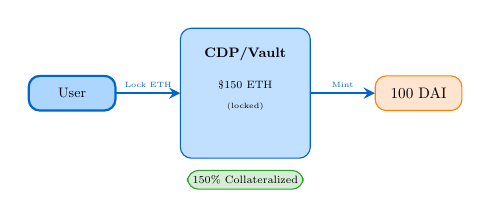
\begin{tikzpicture}[scale=0.55, transform shape]
    % Vault
    \node[rectangle, draw=dfblue, fill=dflightblue3, minimum width=3cm, minimum height=3cm, rounded corners] (vault) at (0, 0) {};
    \node[font=\small\bfseries] at (0, 0.9) {CDP/Vault};
    \node[font=\scriptsize] at (0, 0.2) {\$150 ETH};
    \node[font=\tiny] at (0, -0.3) {(locked)};

    % User
    \node[smartcontract] (user) at (-4, 0) {User};

    % DAI
    \node[rectangle, draw=dforange, fill=dforange!20, minimum width=2cm, minimum height=0.8cm, rounded corners] (dai) at (4, 0) {100 DAI};

    % Arrows
    \draw[arrow] (user) -- (-1.5, 0) node[midway, above, font=\tiny] {Lock ETH};
    \draw[arrow] (1.5, 0) -- (dai) node[midway, above, font=\tiny] {Mint};

    % Collateral ratio
    \node[rectangle, draw=dfgreen, fill=dfgreen!20, rounded corners, font=\scriptsize] at (0, -2) {150\% Collateralized};
\end{tikzpicture}

\vspace{0.2cm}
\textbf{Advantages:}
\begin{itemize}
    \item Decentralized
    \item Transparent reserves
    \item No counterparty risk
\end{itemize}

\textbf{Disadvantages:}
\begin{itemize}
    \item Capital inefficient
    \item Liquidation risk
    \item Complexity
\end{itemize}
\end{column}
\end{columns}
\end{frame}

\begin{frame}{Algorithmic Stablecoins: The Experiment}
\begin{columns}[T]
\begin{column}{0.48\textwidth}
\textbf{Pure Algorithmic (Failed):}
\begin{itemize}
    \item No collateral backing
    \item Dual-token: stable + governance
    \item Expand supply when above peg
    \item Contract supply when below peg
\end{itemize}

\vspace{0.2cm}
\textbf{The Death Spiral:}
\begin{enumerate}
    \item Price drops below peg
    \item Redemptions spike
    \item Confidence collapses
    \item Governance token crashes
    \item System becomes insolvent
\end{enumerate}
\end{column}

\begin{column}{0.48\textwidth}
\begin{alertblock}{Case Study: UST/LUNA (May 2022)}
\begin{itemize}
    \item Peak market cap: \$18B
    \item Collapsed in 72 hours
    \item \$60B total value destroyed
    \item Triggered crypto contagion
\end{itemize}
\end{alertblock}

\vspace{0.3cm}
\textbf{Hybrid Models (Surviving):}
\begin{itemize}
    \item \textbf{FRAX}: Partially collateralized
    \item Dynamic collateral ratio
    \item More resilient to de-peg
\end{itemize}
\end{column}
\end{columns}
\end{frame}

\begin{frame}{Stablecoin Design Comparison}
\begin{center}
\footnotesize
\begin{tabular}{p{2.5cm}|p{3.2cm}|p{3.2cm}|p{3.2cm}}
\toprule
\textbf{Attribute} & \textbf{Fiat-Backed} & \textbf{Crypto-Collateral} & \textbf{Algorithmic} \\
\midrule
Collateral & Fiat in bank & Crypto (150\%+) & None/Partial \\
Centralization & High & Medium & Low \\
Capital Efficiency & High (1:1) & Low (over-collateral) & High (0 collateral) \\
Scalability & Limited by reserves & Limited by collateral & Theoretically unlimited \\
Peg Stability & Strong & Strong & Weak \\
Regulatory Risk & High & Medium & Low \\
Censorship Risk & High & Low & Very Low \\
\bottomrule
\end{tabular}
\end{center}

\vspace{0.3cm}
\begin{block}{The Stablecoin Trilemma}
\begin{center}
You can optimize for two of three: \textbf{Decentralization}, \textbf{Stability}, \textbf{Capital Efficiency}
\end{center}
\end{block}
\end{frame}

\begin{frame}{De-Peg Events: Historical Analysis}
\begin{center}
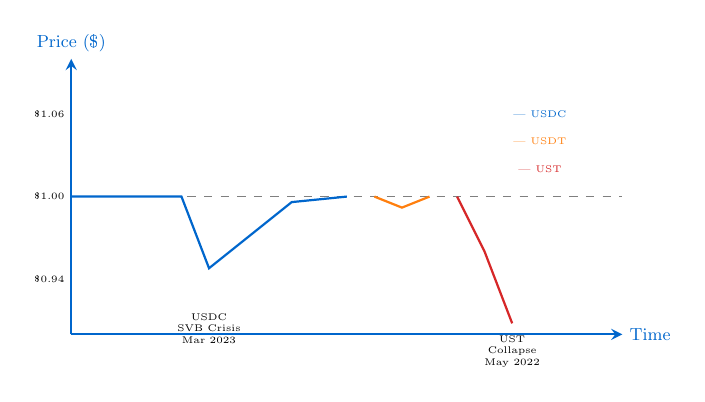
\begin{tikzpicture}[scale=0.7, transform shape]
    % Axes
    \draw[arrow] (0,0) -- (10,0) node[right, font=\small] {Time};
    \draw[arrow] (0,0) -- (0,5) node[above, font=\small] {Price (\$)};

    % Reference line at $1
    \draw[dashed, dfgray] (0, 2.5) -- (10, 2.5);
    \node[left, font=\tiny] at (0, 2.5) {\$1.00};
    \node[left, font=\tiny] at (0, 4) {\$1.06};
    \node[left, font=\tiny] at (0, 1) {\$0.94};

    % USDC de-peg (March 2023)
    \draw[thick, dfblue] (0, 2.5) -- (2, 2.5) -- (2.5, 1.2) -- (4, 2.4) -- (5, 2.5);
    \node[below, font=\tiny, text width=2cm, align=center] at (2.5, 0.5) {USDC\\SVB Crisis\\Mar 2023};

    % USDT de-peg
    \draw[thick, dforange] (5.5, 2.5) -- (6, 2.3) -- (6.5, 2.5);

    % UST collapse
    \draw[thick, dfred] (7, 2.5) -- (7.5, 1.5) -- (8, 0.2);
    \node[below, font=\tiny, text width=2cm, align=center] at (8, 0.1) {UST\\Collapse\\May 2022};

    % Legend
    \node[font=\tiny, dfblue] at (8.5, 4) {--- USDC};
    \node[font=\tiny, dforange] at (8.5, 3.5) {--- USDT};
    \node[font=\tiny, dfred] at (8.5, 3) {--- UST};
\end{tikzpicture}
\end{center}

\textbf{Key Lessons:}
\begin{itemize}
    \item Fiat-backed: Banking system dependencies (SVB, Silvergate)
    \item Algorithmic: Fundamental design flaws lead to death spirals
    \item All designs: Confidence is fragile and self-reinforcing
\end{itemize}
\end{frame}

\begin{frame}{Stablecoin Regulation}
\begin{columns}[T]
\begin{column}{0.48\textwidth}
\textbf{Why Regulators Care:}
\begin{itemize}
    \item Systemic risk (too big to fail?)
    \item Consumer protection
    \item Money laundering concerns
    \item Monetary policy implications
    \item Bank-like activities
\end{itemize}

\vspace{0.3cm}
\textbf{Regulatory Developments:}
\begin{itemize}
    \item EU: MiCA framework (2024)
    \item US: Congressional debate ongoing
    \item Singapore: Clear framework
    \item China: Banned
\end{itemize}
\end{column}

\begin{column}{0.48\textwidth}
\begin{block}{Key Requirements Emerging}
\begin{itemize}
    \item 1:1 reserve backing
    \item Regular audits/attestations
    \item Redemption guarantees
    \item Segregated reserves
    \item Licensing requirements
\end{itemize}
\end{block}

\vspace{0.3cm}
\textbf{Impact on Market:}
\begin{itemize}
    \item USDC: Embracing regulation
    \item USDT: Offshore strategy
    \item DAI: Decentralization defense
\end{itemize}
\end{column}
\end{columns}
\end{frame}

\begin{frame}{Key Competency Check: Stablecoins}
\begin{block}{You should be able to:}
\begin{enumerate}
    \item Classify stablecoins by design type (fiat-backed, crypto-collateralized, algorithmic)
    \item Explain the tradeoffs of each design approach
    \item Assess de-peg risk factors for different stablecoins
    \item Articulate why stablecoins face heavy regulatory scrutiny
\end{enumerate}
\end{block}

\vspace{0.5cm}
\begin{center}
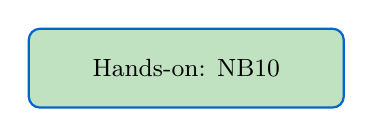
\begin{tikzpicture}
    \node[smartcontract, minimum width=4cm, minimum height=1cm, fill=dfgreen!30] {Hands-on: NB10};
\end{tikzpicture}
\end{center}

\textbf{NB10}: Analyze stablecoin price stability data---examine de-peg events and compare resilience across designs.

\bottomnote{Hands-on: NB10 -- Stablecoin price stability analysis}
\end{frame}

% =====================================================================
% SECTION 4.4: TOKENIZATION AND CBDCs
% =====================================================================
\section{4.4 Tokenization and CBDCs}

\begin{frame}{What is Tokenization?}
\begin{columns}[T]
\begin{column}{0.55\textwidth}
\begin{block}{Definition}
\textbf{Tokenization} is the process of creating a digital representation of a real-world asset on a blockchain.
\end{block}

\vspace{0.3cm}
\textbf{What Can Be Tokenized:}
\begin{itemize}
    \item Real estate
    \item Securities (stocks, bonds)
    \item Commodities (gold, oil)
    \item Art and collectibles
    \item Intellectual property
    \item Carbon credits
\end{itemize}
\end{column}

\begin{column}{0.42\textwidth}
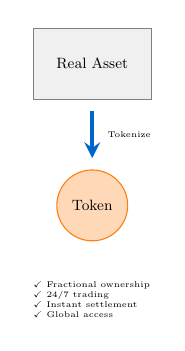
\begin{tikzpicture}[scale=0.6, transform shape]
    % Real asset
    \node[rectangle, draw=dfgray, fill=lightgray, minimum width=2.5cm, minimum height=1.5cm] (asset) at (0, 2.5) {};
    \node[font=\small] at (0, 2.5) {Real Asset};

    % Arrow
    \draw[arrow, line width=1.5pt] (0, 1.5) -- (0, 0.5);
    \node[right, font=\tiny] at (0.2, 1) {Tokenize};

    % Token
    \node[circle, draw=dforange, fill=dforange!30, minimum size=1.5cm] (token) at (0, -0.5) {};
    \node[font=\small] at (0, -0.5) {Token};

    % Benefits
    \node[font=\tiny, text width=2.5cm, align=left] at (0, -2.5) {
        $\checkmark$ Fractional ownership\\
        $\checkmark$ 24/7 trading\\
        $\checkmark$ Instant settlement\\
        $\checkmark$ Global access
    };
\end{tikzpicture}
\end{column}
\end{columns}
\end{frame}

\begin{frame}{Real-World Asset (RWA) Tokenization}
\begin{center}
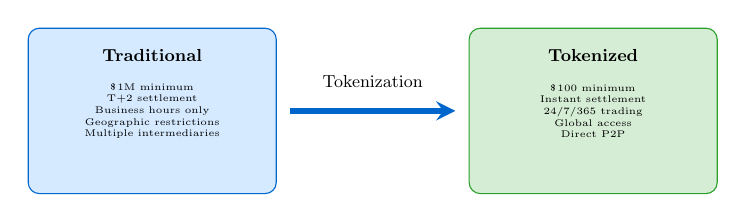
\begin{tikzpicture}[scale=0.7, transform shape]
    % Traditional
    \node[rectangle, draw=dfblue, fill=dflightblue4, minimum width=4.5cm, minimum height=3cm, rounded corners] (trad) at (-4, 0) {};
    \node[font=\small\bfseries] at (-4, 1) {Traditional};
    \node[font=\tiny, text width=4cm, align=center] at (-4, 0) {
        \$1M minimum\\
        T+2 settlement\\
        Business hours only\\
        Geographic restrictions\\
        Multiple intermediaries
    };

    % Arrow
    \draw[arrow, line width=2pt] (-1.5, 0) -- (1.5, 0);
    \node[above, font=\small] at (0, 0.3) {Tokenization};

    % Tokenized
    \node[rectangle, draw=dfgreen, fill=dfgreen!20, minimum width=4.5cm, minimum height=3cm, rounded corners] (tok) at (4, 0) {};
    \node[font=\small\bfseries] at (4, 1) {Tokenized};
    \node[font=\tiny, text width=4cm, align=center] at (4, 0) {
        \$100 minimum\\
        Instant settlement\\
        24/7/365 trading\\
        Global access\\
        Direct P2P
    };
\end{tikzpicture}
\end{center}

\vspace{0.3cm}
\textbf{Market Size Projections:}
\begin{itemize}
    \item Boston Consulting Group: \$16 trillion by 2030
    \item BlackRock, JP Morgan actively building infrastructure
    \item US Treasuries on-chain: \$1B+ (2024)
\end{itemize}
\end{frame}

\begin{frame}{RWA Tokenization Examples}
\begin{center}
\footnotesize
\begin{tabular}{p{2.5cm}|p{3cm}|p{3cm}|p{3.5cm}}
\toprule
\textbf{Asset Class} & \textbf{Example} & \textbf{Platform} & \textbf{Value Proposition} \\
\midrule
Real Estate & Tokenized apartments & RealT, Lofty & Fractional ownership, rental income \\
\addlinespace
US Treasuries & T-bills on-chain & Ondo, Franklin Templeton & DeFi-compatible yield \\
\addlinespace
Private Credit & Corporate loans & Centrifuge, Goldfinch & Access to institutional yields \\
\addlinespace
Commodities & Gold tokens & Paxos Gold (PAXG) & Redeemable for physical \\
\addlinespace
Art & Fractionalized art & Masterworks & Access to blue-chip art \\
\bottomrule
\end{tabular}
\end{center}

\vspace{0.3cm}
\begin{alertblock}{The Legal Challenge}
Tokens represent claims on assets, but enforcement still requires legal systems. ``Code is law'' doesn't apply when real-world assets need real-world courts.
\end{alertblock}
\end{frame}

\begin{frame}{Central Bank Digital Currencies (CBDCs)}
\begin{columns}[T]
\begin{column}{0.55\textwidth}
\begin{block}{Definition}
A \textbf{CBDC} is a digital form of central bank money, denominated in the national unit of account and a direct liability of the central bank.
\end{block}

\vspace{0.3cm}
\textbf{Global Status (2024):}
\begin{itemize}
    \item 130+ countries exploring
    \item 3 fully launched (Bahamas, Nigeria, Jamaica)
    \item 20+ in pilot phase
    \item Major economies in research
\end{itemize}
\end{column}

\begin{column}{0.42\textwidth}
\textbf{Two Main Types:}

\vspace{0.2cm}
\textbf{Retail CBDC:}
\begin{itemize}
    \item For general public
    \item Replaces/complements cash
    \item Direct central bank relationship
\end{itemize}

\vspace{0.2cm}
\textbf{Wholesale CBDC:}
\begin{itemize}
    \item For financial institutions
    \item Interbank settlements
    \item Less disruptive to banking
\end{itemize}
\end{column}
\end{columns}
\end{frame}

\begin{frame}{CBDC Architecture Models}
\begin{center}
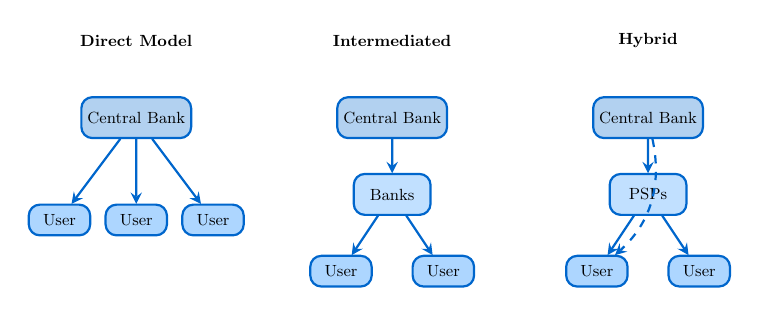
\begin{tikzpicture}[scale=0.65, transform shape]
    % Model 1: Direct
    \node[font=\small\bfseries] at (-5, 3) {Direct Model};
    \node[smartcontract, minimum width=2cm, fill=dfblue!30] (cb1) at (-5, 1.5) {Central Bank};
    \node[smartcontract, minimum width=1.2cm, minimum height=0.6cm] (u1a) at (-6.5, -0.5) {User};
    \node[smartcontract, minimum width=1.2cm, minimum height=0.6cm] (u1b) at (-5, -0.5) {User};
    \node[smartcontract, minimum width=1.2cm, minimum height=0.6cm] (u1c) at (-3.5, -0.5) {User};
    \draw[arrow] (cb1) -- (u1a);
    \draw[arrow] (cb1) -- (u1b);
    \draw[arrow] (cb1) -- (u1c);

    % Model 2: Intermediated
    \node[font=\small\bfseries] at (0, 3) {Intermediated};
    \node[smartcontract, minimum width=2cm, fill=dfblue!30] (cb2) at (0, 1.5) {Central Bank};
    \node[smartcontract, minimum width=1.5cm, fill=dflightblue3] (bank2) at (0, 0) {Banks};
    \node[smartcontract, minimum width=1.2cm, minimum height=0.6cm] (u2a) at (-1, -1.5) {User};
    \node[smartcontract, minimum width=1.2cm, minimum height=0.6cm] (u2b) at (1, -1.5) {User};
    \draw[arrow] (cb2) -- (bank2);
    \draw[arrow] (bank2) -- (u2a);
    \draw[arrow] (bank2) -- (u2b);

    % Model 3: Hybrid
    \node[font=\small\bfseries] at (5, 3) {Hybrid};
    \node[smartcontract, minimum width=2cm, fill=dfblue!30] (cb3) at (5, 1.5) {Central Bank};
    \node[smartcontract, minimum width=1.5cm, fill=dflightblue3] (psp) at (5, 0) {PSPs};
    \node[smartcontract, minimum width=1.2cm, minimum height=0.6cm] (u3a) at (4, -1.5) {User};
    \node[smartcontract, minimum width=1.2cm, minimum height=0.6cm] (u3b) at (6, -1.5) {User};
    \draw[arrow] (cb3) -- (psp);
    \draw[arrow, dashed] (cb3) to[bend left=30] (u3a);
    \draw[arrow] (psp) -- (u3a);
    \draw[arrow] (psp) -- (u3b);
\end{tikzpicture}
\end{center}

\vspace{0.2cm}
\textbf{Trade-offs:}
\begin{itemize}
    \item Direct: Maximum control, but central bank becomes retail bank
    \item Intermediated: Preserves banking system, but less innovative
    \item Hybrid: Balance, but complex implementation
\end{itemize}
\end{frame}

\begin{frame}{CBDC vs. Stablecoin Comparison}
\begin{center}
\footnotesize
\begin{tabular}{p{3cm}|p{4.5cm}|p{4.5cm}}
\toprule
\textbf{Attribute} & \textbf{CBDC} & \textbf{Stablecoin} \\
\midrule
Issuer & Central bank (sovereign) & Private company \\
Liability & Central bank balance sheet & Private balance sheet \\
Legal Status & Legal tender & Private money \\
Backing & Full faith of government & Reserves (varies) \\
Programmability & Policy-controlled & Open/permissionless \\
Privacy & Policy-dependent & Pseudonymous (public chains) \\
Innovation Speed & Slow (government) & Fast (private) \\
Interoperability & National focus & Global by default \\
Risk Profile & Sovereign risk only & Counterparty + operational \\
\bottomrule
\end{tabular}
\end{center}

\vspace{0.2cm}
\begin{block}{Key Question}
Will CBDCs complement, compete with, or regulate away private stablecoins?
\end{block}
\end{frame}

\begin{frame}{Programmable Money: The Convergence}
\begin{columns}[T]
\begin{column}{0.48\textwidth}
\textbf{What Programmability Enables:}
\begin{itemize}
    \item Conditional payments
    \item Automatic tax withholding
    \item Stimulus with expiration dates
    \item Supply chain financing
    \item Smart contract integration
\end{itemize}

\vspace{0.3cm}
\textbf{Opportunities:}
\begin{itemize}
    \item Financial inclusion
    \item Reduced fraud
    \item Efficient policy transmission
    \item New business models
\end{itemize}
\end{column}

\begin{column}{0.48\textwidth}
\begin{alertblock}{Concerns}
\begin{itemize}
    \item \textbf{Privacy}: Complete transaction surveillance
    \item \textbf{Control}: Money that ``expires'' or can be frozen
    \item \textbf{Exclusion}: Programmable discrimination
    \item \textbf{Security}: Single point of failure
\end{itemize}
\end{alertblock}

\vspace{0.2cm}
\textbf{Design Choices Matter:}
\begin{itemize}
    \item Token-based vs. account-based
    \item Privacy-preserving tech
    \item Offline capability
    \item Holding limits
\end{itemize}
\end{column}
\end{columns}
\end{frame}

\begin{frame}{The Tokenization Landscape}
\begin{center}
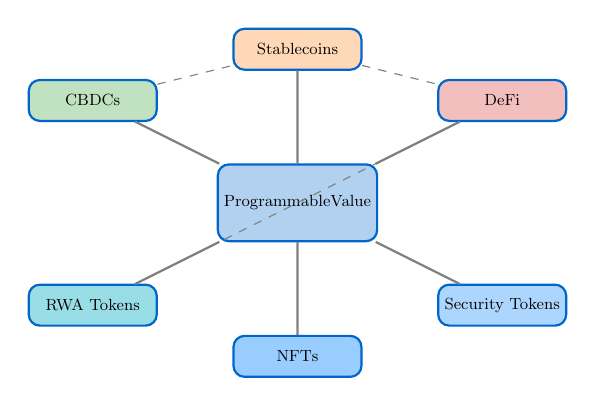
\begin{tikzpicture}[scale=0.65, transform shape]
    % Central concept
    \node[smartcontract, minimum width=3cm, minimum height=1.5cm, fill=dfblue!30] (center) at (0, 0) {Programmable\\Value};

    % Surrounding concepts
    \node[smartcontract, minimum width=2.5cm, fill=dfgreen!30] (cbdc) at (-4, 2) {CBDCs};
    \node[smartcontract, minimum width=2.5cm, fill=dforange!30] (stable) at (0, 3) {Stablecoins};
    \node[smartcontract, minimum width=2.5cm, fill=dfred!30] (defi) at (4, 2) {DeFi};
    \node[smartcontract, minimum width=2.5cm, fill=dfcyan!50] (rwa) at (-4, -2) {RWA Tokens};
    \node[smartcontract, minimum width=2.5cm, fill=dflightblue] (nft) at (0, -3) {NFTs};
    \node[smartcontract, minimum width=2.5cm, fill=dflightblue2] (sec) at (4, -2) {Security Tokens};

    % Connections
    \draw[thick, dfgray] (center) -- (cbdc);
    \draw[thick, dfgray] (center) -- (stable);
    \draw[thick, dfgray] (center) -- (defi);
    \draw[thick, dfgray] (center) -- (rwa);
    \draw[thick, dfgray] (center) -- (nft);
    \draw[thick, dfgray] (center) -- (sec);

    % Cross connections
    \draw[dashed, dfgray] (stable) -- (defi);
    \draw[dashed, dfgray] (rwa) -- (defi);
    \draw[dashed, dfgray] (cbdc) -- (stable);
\end{tikzpicture}
\end{center}

\textbf{The Convergence Thesis:} Traditional finance (TradFi) and decentralized finance (DeFi) are converging. The future is not ``either/or'' but hybrid systems combining the best of both.
\end{frame}

\begin{frame}{Key Competency Check: Tokenization and CBDCs}
\begin{block}{You should be able to:}
\begin{enumerate}
    \item Explain the mechanics and value proposition of RWA tokenization
    \item Compare different CBDC architectural models
    \item Evaluate the tradeoffs between CBDCs and stablecoins
    \item Assess the implications of programmable sovereign money
\end{enumerate}
\end{block}

\vspace{0.5cm}
\begin{block}{Discussion Questions}
\begin{itemize}
    \item Should central banks issue retail CBDCs? What are the risks?
    \item Will tokenization democratize access to investments or create new risks?
    \item How should programmable money be governed?
\end{itemize}
\end{block}
\end{frame}

% =====================================================================
% SUMMARY AND WRAP-UP
% =====================================================================
\section*{Day 4 Summary}

\begin{frame}{Day 4: Key Takeaways}
\begin{columns}[T]
\begin{column}{0.48\textwidth}
\textbf{4.1 Smart Contracts:}
\begin{itemize}
    \item Self-executing code on blockchain
    \item ``Trustless'' shifts trust, doesn't eliminate it
    \item Oracle problem limits external data access
\end{itemize}

\vspace{0.3cm}
\textbf{4.2 DeFi Primitives:}
\begin{itemize}
    \item AMMs use $x \cdot y = k$ for pricing
    \item Impermanent loss affects liquidity providers
    \item Composability enables innovation (and attacks)
\end{itemize}
\end{column}

\begin{column}{0.48\textwidth}
\textbf{4.3 Stablecoins:}
\begin{itemize}
    \item Three designs: fiat-backed, crypto-collateral, algorithmic
    \item Stablecoin trilemma constrains design
    \item Heavy regulatory focus globally
\end{itemize}

\vspace{0.3cm}
\textbf{4.4 Tokenization \& CBDCs:}
\begin{itemize}
    \item RWA tokenization unlocks liquidity
    \item CBDCs represent sovereign response
    \item Programmable money raises privacy concerns
\end{itemize}
\end{column}
\end{columns}
\end{frame}

\begin{frame}{Hands-On Notebooks for Day 4}
\begin{center}
\begin{tabular}{p{2cm}|p{5cm}|p{5cm}}
\toprule
\textbf{Notebook} & \textbf{Topic} & \textbf{Key Activities} \\
\midrule
NB08 & Smart Contract Interaction & Interact with contracts on testnet, call functions, observe state changes \\
\addlinespace
NB09 & AMM Simulation & Provide liquidity, execute swaps, measure impermanent loss \\
\addlinespace
NB10 & Stablecoin Analysis & Analyze price stability data, examine de-peg events \\
\bottomrule
\end{tabular}
\end{center}

\vspace{0.5cm}
\begin{block}{Preparation for Day 5}
Tomorrow we explore the \textbf{AI-Finance Intersection}: Machine learning for markets, LLMs in finance, and the automation of financial decisions.
\end{block}
\end{frame}

\begin{frame}{Questions?}
\begin{center}
\vspace{1cm}
{\Huge Day 4: Programmable Finance}

\vspace{0.5cm}
{\large Smart Contracts, DeFi, and Tokenization}

\vspace{1cm}
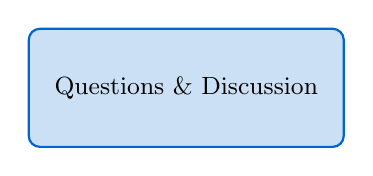
\begin{tikzpicture}
    \node[smartcontract, minimum width=4cm, minimum height=1.5cm, fill=dfblue!20] {Questions \& Discussion};
\end{tikzpicture}

\vspace{1cm}
\textbf{Next:} Day 5 -- AI and Finance
\end{center}
\end{frame}

\end{document}
